\documentclass[11pt]{article}\usepackage[]{graphicx}\usepackage[]{xcolor}
% maxwidth is the original width if it is less than linewidth
% otherwise use linewidth (to make sure the graphics do not exceed the margin)
\makeatletter
\def\maxwidth{ %
  \ifdim\Gin@nat@width>\linewidth
    \linewidth
  \else
    \Gin@nat@width
  \fi
}
\makeatother

\definecolor{fgcolor}{rgb}{0.345, 0.345, 0.345}
\newcommand{\hlnum}[1]{\textcolor[rgb]{0.686,0.059,0.569}{#1}}%
\newcommand{\hlstr}[1]{\textcolor[rgb]{0.192,0.494,0.8}{#1}}%
\newcommand{\hlcom}[1]{\textcolor[rgb]{0.678,0.584,0.686}{\textit{#1}}}%
\newcommand{\hlopt}[1]{\textcolor[rgb]{0,0,0}{#1}}%
\newcommand{\hlstd}[1]{\textcolor[rgb]{0.345,0.345,0.345}{#1}}%
\newcommand{\hlkwa}[1]{\textcolor[rgb]{0.161,0.373,0.58}{\textbf{#1}}}%
\newcommand{\hlkwb}[1]{\textcolor[rgb]{0.69,0.353,0.396}{#1}}%
\newcommand{\hlkwc}[1]{\textcolor[rgb]{0.333,0.667,0.333}{#1}}%
\newcommand{\hlkwd}[1]{\textcolor[rgb]{0.737,0.353,0.396}{\textbf{#1}}}%
\let\hlipl\hlkwb

\usepackage{framed}
\makeatletter
\newenvironment{kframe}{%
 \def\at@end@of@kframe{}%
 \ifinner\ifhmode%
  \def\at@end@of@kframe{\end{minipage}}%
  \begin{minipage}{\columnwidth}%
 \fi\fi%
 \def\FrameCommand##1{\hskip\@totalleftmargin \hskip-\fboxsep
 \colorbox{shadecolor}{##1}\hskip-\fboxsep
     % There is no \\@totalrightmargin, so:
     \hskip-\linewidth \hskip-\@totalleftmargin \hskip\columnwidth}%
 \MakeFramed {\advance\hsize-\width
   \@totalleftmargin\z@ \linewidth\hsize
   \@setminipage}}%
 {\par\unskip\endMakeFramed%
 \at@end@of@kframe}
\makeatother

\definecolor{shadecolor}{rgb}{.97, .97, .97}
\definecolor{messagecolor}{rgb}{0, 0, 0}
\definecolor{warningcolor}{rgb}{1, 0, 1}
\definecolor{errorcolor}{rgb}{1, 0, 0}
\newenvironment{knitrout}{}{} % an empty environment to be redefined in TeX

\usepackage{alltt}

% Packages for graphics & layout
\usepackage{graphicx}
\usepackage{epstopdf}
\usepackage{caption}
\usepackage{subcaption}
\usepackage{booktabs}
\usepackage[a4paper,margin=0.5in]{geometry}
\usepackage{lipsum}
\usepackage{multicol}

\usepackage[utf8]{inputenc}
\usepackage{enumitem}

% Packages for math
\usepackage{amsmath}
\usepackage{amsfonts}
\usepackage{amssymb}

% Package for bibliography
\usepackage{natbib}
\usepackage{hyperref}

% listing setup \usepackage{listings}
\usepackage{color} % For syntax highlighting color
\captionsetup{labelfont=bf}
\setlength{\parskip}{0.5\baselineskip}


\title{\textbf{Data Analysis Practice}}
\author{Michael V Cumbo}
\date{\today}
\IfFileExists{upquote.sty}{\usepackage{upquote}}{}
\begin{document}
\maketitle
\section*{Objective}
Explore the relationship between miles per gallon (\textit{mpg}) and other variables in the \texttt{mtcars} dataset.

\section*{Tasks}

\subsection*{1. Load the \texttt{mtcars} Dataset}
\begin{itemize}
    \item Start by loading the \texttt{mtcars} dataset into R. This dataset comes pre-loaded in R, so you don't need to download it from anywhere. Just use \texttt{data(mtcars)} to load it.
\end{itemize}
\subsection*{2. Basic Exploration}
\begin{itemize}
    \item Display the first few rows of the dataset using the \texttt{head()} function.
    \item Use the \texttt{summary()} function to get a summary of the dataset.
\end{itemize}
\begin{knitrout}
\definecolor{shadecolor}{rgb}{0.969, 0.969, 0.969}\color{fgcolor}\begin{kframe}
\begin{alltt}
\hlkwd{library}\hlstd{(tidyverse)}
\hlkwd{library}\hlstd{(dplyr)}

\hlstd{mtcars} \hlkwb{<-} \hlstd{mtcars}

\hlkwd{head}\hlstd{(mtcars)}
\end{alltt}
\begin{verbatim}
##                    mpg cyl disp  hp drat    wt  qsec vs am gear carb
## Mazda RX4         21.0   6  160 110 3.90 2.620 16.46  0  1    4    4
## Mazda RX4 Wag     21.0   6  160 110 3.90 2.875 17.02  0  1    4    4
## Datsun 710        22.8   4  108  93 3.85 2.320 18.61  1  1    4    1
## Hornet 4 Drive    21.4   6  258 110 3.08 3.215 19.44  1  0    3    1
## Hornet Sportabout 18.7   8  360 175 3.15 3.440 17.02  0  0    3    2
## Valiant           18.1   6  225 105 2.76 3.460 20.22  1  0    3    1
##                   mpg_category
## Mazda RX4             High MPG
## Mazda RX4 Wag         High MPG
## Datsun 710            High MPG
## Hornet 4 Drive        High MPG
## Hornet Sportabout      Low MPG
## Valiant                Low MPG
\end{verbatim}
\end{kframe}
\end{knitrout}
\clearpage
\begin{knitrout}
\definecolor{shadecolor}{rgb}{0.969, 0.969, 0.969}\color{fgcolor}\begin{kframe}
\begin{alltt}
\hlstd{mtcars} \hlopt
  \hlkwd{summary}\hlstd{()}
\end{alltt}
\begin{verbatim}
##       mpg             cyl             disp             hp       
##  Min.   :10.40   Min.   :4.000   Min.   : 71.1   Min.   : 52.0  
##  1st Qu.:15.43   1st Qu.:4.000   1st Qu.:120.8   1st Qu.: 96.5  
##  Median :19.20   Median :6.000   Median :196.3   Median :123.0  
##  Mean   :20.09   Mean   :6.188   Mean   :230.7   Mean   :146.7  
##  3rd Qu.:22.80   3rd Qu.:8.000   3rd Qu.:326.0   3rd Qu.:180.0  
##  Max.   :33.90   Max.   :8.000   Max.   :472.0   Max.   :335.0  
##       drat             wt             qsec             vs        
##  Min.   :2.760   Min.   :1.513   Min.   :14.50   Min.   :0.0000  
##  1st Qu.:3.080   1st Qu.:2.581   1st Qu.:16.89   1st Qu.:0.0000  
##  Median :3.695   Median :3.325   Median :17.71   Median :0.0000  
##  Mean   :3.597   Mean   :3.217   Mean   :17.85   Mean   :0.4375  
##  3rd Qu.:3.920   3rd Qu.:3.610   3rd Qu.:18.90   3rd Qu.:1.0000  
##  Max.   :4.930   Max.   :5.424   Max.   :22.90   Max.   :1.0000  
##        am              gear            carb       mpg_category      
##  Min.   :0.0000   Min.   :3.000   Min.   :1.000   Length:32         
##  1st Qu.:0.0000   1st Qu.:3.000   1st Qu.:2.000   Class :character  
##  Median :0.0000   Median :4.000   Median :2.000   Mode  :character  
##  Mean   :0.4062   Mean   :3.688   Mean   :2.812                     
##  3rd Qu.:1.0000   3rd Qu.:4.000   3rd Qu.:4.000                     
##  Max.   :1.0000   Max.   :5.000   Max.   :8.000
\end{verbatim}
\end{kframe}
\end{knitrout}
\subsection*{3. Data Analysis}
\begin{itemize}
    \item Create a new column in the dataset that categorizes cars into "High MPG" and "Low MPG" based on whether their \textit{mpg} is above or below the median \textit{mpg} of all cars in the dataset. You can use the \texttt{ifelse()} function for this.
\end{itemize}
\begin{knitrout}
\definecolor{shadecolor}{rgb}{0.969, 0.969, 0.969}\color{fgcolor}\begin{kframe}
\begin{alltt}
\hlstd{mtcars} \hlkwb{<-} \hlstd{mtcars} \hlopt
  \hlkwd{mutate}\hlstd{(}\hlkwc{mpg_category} \hlstd{=} \hlkwd{ifelse}\hlstd{(mpg} \hlopt{>} \hlnum{20.09}\hlstd{,} \hlstr{"High MPG"}\hlstd{,} \hlstr{"Low MPG"}\hlstd{))}
\end{alltt}
\end{kframe}
\end{knitrout}
\clearpage
\subsection*{4. Visualization}
\begin{itemize}
    \item Plot a histogram of \textit{mpg} to see its distribution.
    \item Create a scatter plot to examine the relationship between \textit{mpg} and weight (\texttt{wt}). 
    \item Bonus: Color the points in your scatter plot based on the "High MPG" and "Low MPG" categorization.
\end{itemize}

\begin{knitrout}
\definecolor{shadecolor}{rgb}{0.969, 0.969, 0.969}\color{fgcolor}\begin{kframe}
\begin{alltt}
\hlkwd{hist}\hlstd{(mtcars}\hlopt{$}\hlstd{mpg)}
\end{alltt}
\end{kframe}
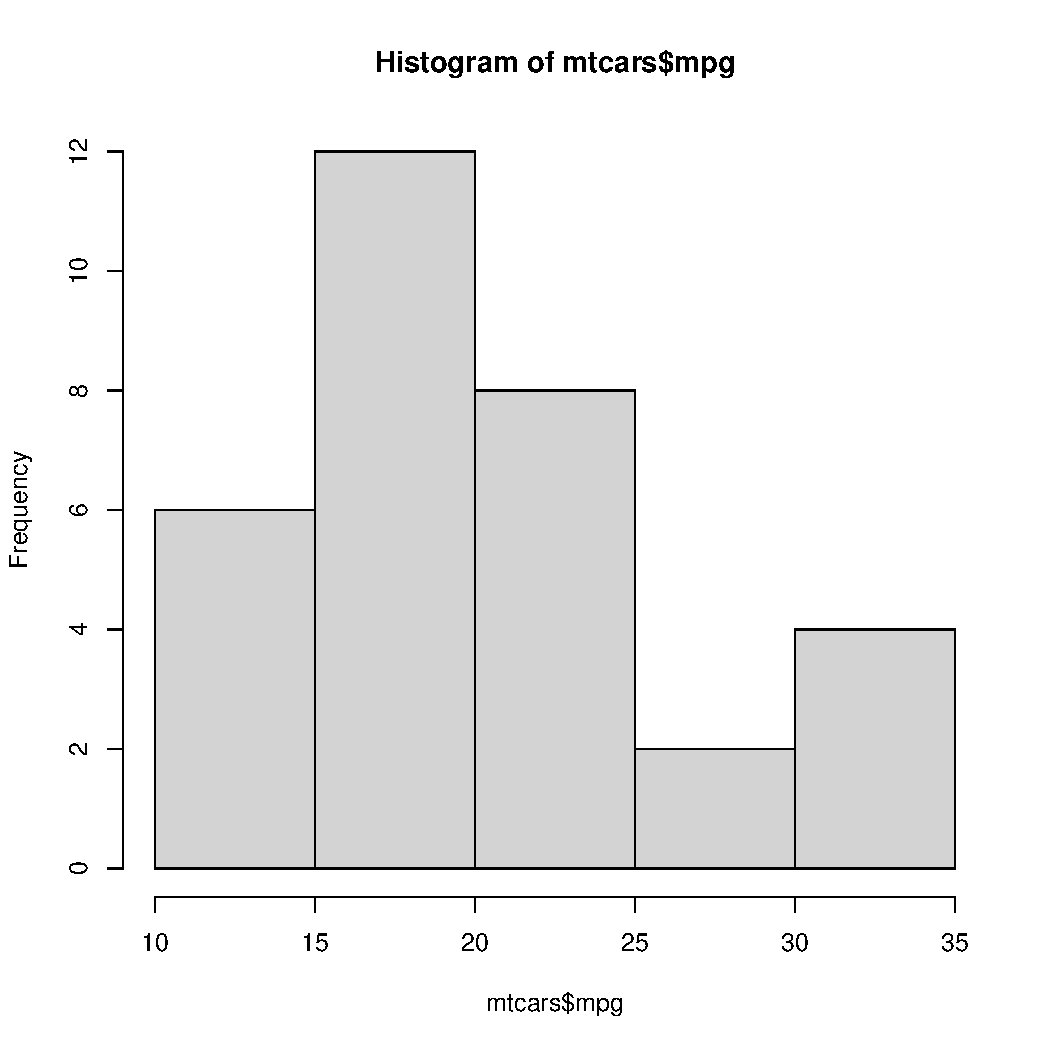
\includegraphics[width=\maxwidth]{figure/Q4-1} 
\begin{kframe}\begin{alltt}
\hlkwd{plot}\hlstd{(mtcars}\hlopt{$}\hlstd{wt, mtcars}\hlopt{$}\hlstd{mpg)}
\end{alltt}
\end{kframe}
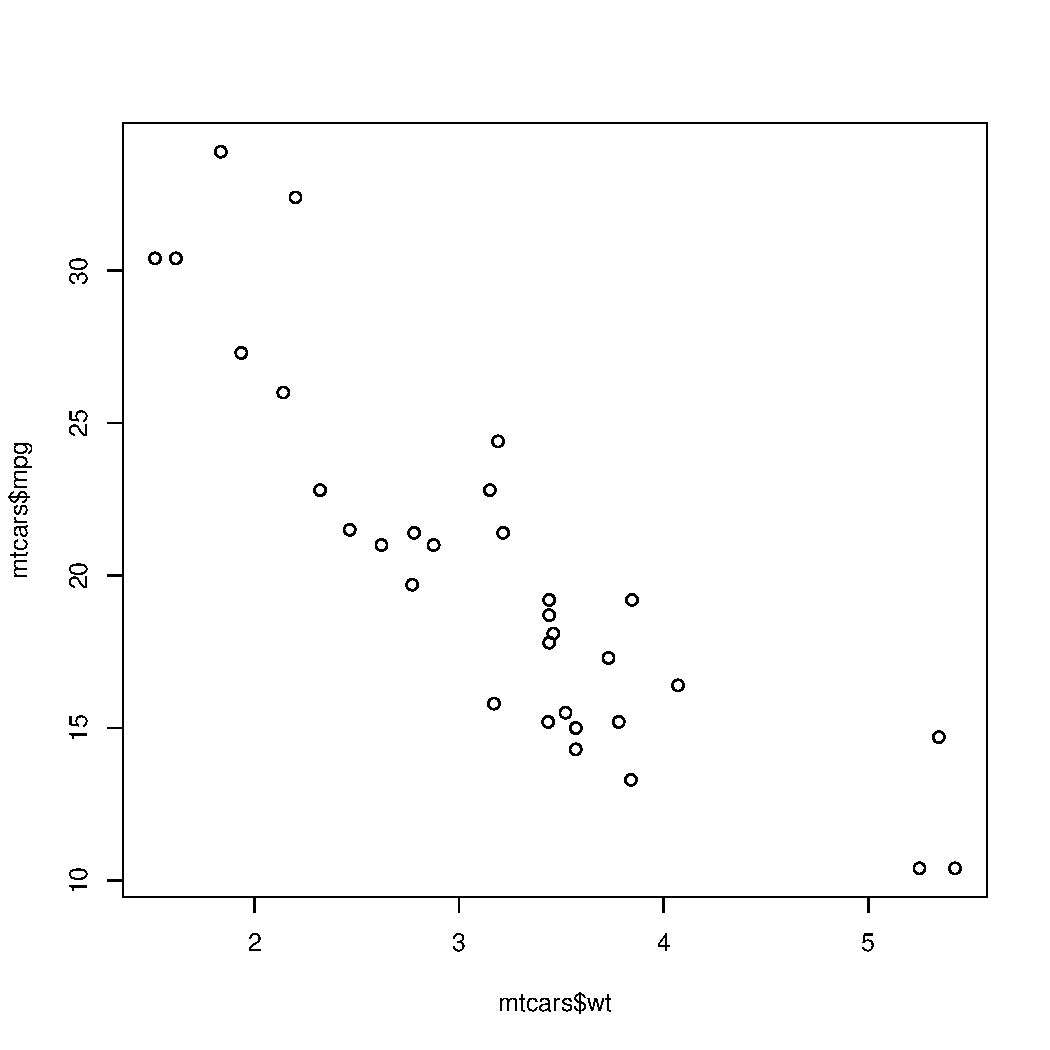
\includegraphics[width=\maxwidth]{figure/Q4-2} 
\end{knitrout}
\clearpage
\subsection*{5. Advanced Analysis (Optional)}
\begin{itemize}
    \item Perform a linear regression analysis to study the relationship between \textit{mpg} (as the dependent variable) and other variables like weight (\texttt{wt}), horsepower (\texttt{hp}), and number of cylinders (\texttt{cyl}). Use the \texttt{lm()} function for this.
    \item Summarize your linear regression model using the \texttt{summary()} function and interpret the results.
\end{itemize}
\begin{knitrout}
\definecolor{shadecolor}{rgb}{0.969, 0.969, 0.969}\color{fgcolor}\begin{kframe}
\begin{alltt}
\hlkwd{library}\hlstd{(tidyverse)}
\hlcom{# Define the independent variables}
\hlstd{independent_vars} \hlkwb{<-} \hlkwd{c}\hlstd{(}\hlstr{"hp"}\hlstd{,} \hlstr{"cyl"}\hlstd{,} \hlstr{"drat"}\hlstd{,} \hlstr{"qsec"}\hlstd{,} \hlstr{"vs"}\hlstd{,} \hlstr{"carb"}\hlstd{)}
\hlcom{# Create a list of formulas}
\hlstd{formulas} \hlkwb{<-} \hlkwd{lapply}\hlstd{(}
  \hlstd{independent_vars,}
  \hlkwa{function}\hlstd{(}\hlkwc{var}\hlstd{)} \hlkwd{as.formula}\hlstd{(}\hlkwd{paste}\hlstd{(}\hlstr{"mpg ~"}\hlstd{, var))}
\hlstd{)}
\hlcom{# Use map() to apply lm() to each formula}
\hlstd{models} \hlkwb{<-} \hlkwd{map}\hlstd{(formulas,} \hlopt{~} \hlkwd{lm}\hlstd{(}\hlkwc{data} \hlstd{= mtcars,} \hlkwc{formula} \hlstd{= .))}
\hlcom{# Create a tibble with model summaries}
\hlstd{model_summaries} \hlkwb{<-} \hlkwd{tibble}\hlstd{(}\hlkwc{variable} \hlstd{= independent_vars,} \hlkwc{model} \hlstd{= models)} \hlopt
  \hlkwd{mutate}\hlstd{(}\hlkwc{summary} \hlstd{=} \hlkwd{map}\hlstd{(model, summary))}
\hlcom{# View the tibble}
\hlkwd{print}\hlstd{(model_summaries)}
\end{alltt}
\begin{verbatim}
## # A tibble: 6 x 3
##   variable model  summary   
##   <chr>    <list> <list>    
## 1 hp       <lm>   <smmry.lm>
## 2 cyl      <lm>   <smmry.lm>
## 3 drat     <lm>   <smmry.lm>
## 4 qsec     <lm>   <smmry.lm>
## 5 vs       <lm>   <smmry.lm>
## 6 carb     <lm>   <smmry.lm>
\end{verbatim}
\begin{alltt}
\hlcom{# Extract and print the summary}
\hlcom{# for the model with 'hp' as the independent variable}
\hlstd{hp_model_summary} \hlkwb{<-} \hlstd{model_summaries} \hlopt
  \hlkwd{filter}\hlstd{(variable} \hlopt{==} \hlstr{"hp"}\hlstd{)} \hlopt
  \hlkwd{pull}\hlstd{(summary)}
\hlcom{# Display the summary}
\hlkwd{print}\hlstd{(hp_model_summary)}
\end{alltt}
\begin{verbatim}
## 
## Call:
## lm(formula = ., data = mtcars)
## 
## Residuals:
##     Min      1Q  Median      3Q 
## -5.7121 -2.1122 -0.8854  1.5819 
##     Max 
##  8.2360 
## 
## Coefficients:
##             Estimate Std. Error
## (Intercept) 30.09886    1.63392
## hp          -0.06823    0.01012
##             t value Pr(>|t|)    
## (Intercept)  18.421  < 2e-16 ***
## hp           -6.742 1.79e-07 ***
## ---
## Signif. codes:  
##   0 '***' 0.001 '**' 0.01 '*'
##   0.05 '.' 0.1 ' ' 1
## 
## Residual standard error: 3.863 on 30 degrees of freedom
## Multiple R-squared:  0.6024,	Adjusted R-squared:  0.5892 
## F-statistic: 45.46 on 1 and 30 DF,  p-value: 1.788e-07
## 
## 
## Call:
## lm(formula = ., data = mtcars)
## 
## Residuals:
##     Min      1Q  Median      3Q 
## -4.9814 -2.1185  0.2217  1.0717 
##     Max 
##  7.5186 
## 
## Coefficients:
##             Estimate Std. Error
## (Intercept)  37.8846     2.0738
## cyl          -2.8758     0.3224
##             t value Pr(>|t|)    
## (Intercept)   18.27  < 2e-16 ***
## cyl           -8.92 6.11e-10 ***
## ---
## Signif. codes:  
##   0 '***' 0.001 '**' 0.01 '*'
##   0.05 '.' 0.1 ' ' 1
## 
## Residual standard error: 3.206 on 30 degrees of freedom
## Multiple R-squared:  0.7262,	Adjusted R-squared:  0.7171 
## F-statistic: 79.56 on 1 and 30 DF,  p-value: 6.113e-10
## 
## 
## Call:
## lm(formula = ., data = mtcars)
## 
## Residuals:
##     Min      1Q  Median      3Q 
## -9.0775 -2.6803 -0.2095  2.2976 
##     Max 
##  9.0225 
## 
## Coefficients:
##             Estimate Std. Error
## (Intercept)   -7.525      5.477
## drat           7.678      1.507
##             t value Pr(>|t|)    
## (Intercept)  -1.374     0.18    
## drat          5.096 1.78e-05 ***
## ---
## Signif. codes:  
##   0 '***' 0.001 '**' 0.01 '*'
##   0.05 '.' 0.1 ' ' 1
## 
## Residual standard error: 4.485 on 30 degrees of freedom
## Multiple R-squared:  0.464,	Adjusted R-squared:  0.4461 
## F-statistic: 25.97 on 1 and 30 DF,  p-value: 1.776e-05
## 
## 
## Call:
## lm(formula = ., data = mtcars)
## 
## Residuals:
##     Min      1Q  Median      3Q 
## -9.8760 -3.4539 -0.7203  2.2774 
##     Max 
## 11.6491 
## 
## Coefficients:
##             Estimate Std. Error
## (Intercept)  -5.1140    10.0295
## qsec          1.4121     0.5592
##             t value Pr(>|t|)  
## (Intercept)  -0.510   0.6139  
## qsec          2.525   0.0171 *
## ---
## Signif. codes:  
##   0 '***' 0.001 '**' 0.01 '*'
##   0.05 '.' 0.1 ' ' 1
## 
## Residual standard error: 5.564 on 30 degrees of freedom
## Multiple R-squared:  0.1753,	Adjusted R-squared:  0.1478 
## F-statistic: 6.377 on 1 and 30 DF,  p-value: 0.01708
## 
## 
## Call:
## lm(formula = ., data = mtcars)
## 
## Residuals:
##    Min     1Q Median     3Q    Max 
## -6.757 -3.082 -1.267  2.828  9.383 
## 
## Coefficients:
##             Estimate Std. Error
## (Intercept)   16.617      1.080
## vs             7.940      1.632
##             t value Pr(>|t|)    
## (Intercept)  15.390 8.85e-16 ***
## vs            4.864 3.42e-05 ***
## ---
## Signif. codes:  
##   0 '***' 0.001 '**' 0.01 '*'
##   0.05 '.' 0.1 ' ' 1
## 
## Residual standard error: 4.581 on 30 degrees of freedom
## Multiple R-squared:  0.4409,	Adjusted R-squared:  0.4223 
## F-statistic: 23.66 on 1 and 30 DF,  p-value: 3.416e-05
## 
## 
## Call:
## lm(formula = ., data = mtcars)
## 
## Residuals:
##    Min     1Q Median     3Q    Max 
## -7.250 -3.316 -1.433  3.384 10.083 
## 
## Coefficients:
##             Estimate Std. Error
## (Intercept)  25.8723     1.8368
## carb         -2.0557     0.5685
##             t value Pr(>|t|)    
## (Intercept)  14.085 9.22e-15 ***
## carb         -3.616  0.00108 ** 
## ---
## Signif. codes:  
##   0 '***' 0.001 '**' 0.01 '*'
##   0.05 '.' 0.1 ' ' 1
## 
## Residual standard error: 5.113 on 30 degrees of freedom
## Multiple R-squared:  0.3035,	Adjusted R-squared:  0.2803 
## F-statistic: 13.07 on 1 and 30 DF,  p-value: 0.001084
\end{verbatim}
\end{kframe}
\end{knitrout}
\clearpage
\subsection*{6. Reflection}
\begin{itemize}
    \item Write a brief summary of your findings. Which variables seem to affect \textit{mpg} the most? Were there any surprises in your analysis?
\end{itemize}

\section*{Deliverables}
\begin{itemize}
    \item R script with your code and comments explaining each step.
    \item A brief report summarizing your findings.
\end{itemize}

begin{enumerate}
    \item \textbf{Horsepower (hp):}
    \begin{itemize}
        \item Coefficient: $-0.06823$. This indicates that for every unit increase in horsepower, mpg decreases by approximately 0.06823 units.
        \item P-value: $1.79 \times 10^{-7}$, showing a strong negative relationship between horsepower and mpg.
    \end{itemize}

    \item \textbf{Number of Cylinders (cyl):}
    \begin{itemize}
        \item Coefficient: $-2.8758$, suggesting a substantial decrease in mpg with each additional cylinder.
        \item P-value: $6.11 \times 10^{-10}$, indicating a strong inverse relationship between the number of cylinders and mpg.
    \end{itemize}

    \item \textbf{Rear Axle Ratio (drat):}
    \begin{itemize}
        \item Coefficient: $7.678$, showing a positive relationship with mpg.
        \item P-value: $1.78 \times 10^{-5}$, suggesting that cars with higher rear axle ratios tend to have better fuel efficiency.
    \end{itemize}

    \item \textbf{1/4 Mile Time (qsec):}
    \begin{itemize}
        \item Coefficient: $1.4121$, indicating that cars with faster quarter-mile times tend to have slightly higher mpg.
        \item P-value: $0.0171$, though with a lower R-squared value, suggesting a weaker overall model fit.
    \end{itemize}

    \item \textbf{Engine Configuration (vs):}
    \begin{itemize}
        \item Coefficient: $7.940$, showing a strong positive effect on mpg.
        \item P-value: $3.42 \times 10^{-5}$, indicating that engine configuration has a notable impact on fuel efficiency.
    \end{itemize}

    \item \textbf{Number of Carburetors (carb):}
    \begin{itemize}
        \item Coefficient: $-2.0557$, suggesting that more carburetors are associated with lower mpg.
        \item P-value: $0.00108$.
    \end{itemize}
\end{enumerate}

In conclusion, the number of cylinders (\texttt{cyl}) and horsepower (\texttt{hp}) show the strongest negative relationships with mpg, indicating that cars with more cylinders and higher horsepower tend to have lower fuel efficiency. Conversely, the rear axle ratio (\texttt{drat}) and engine configuration (\texttt{vs}) positively impact mpg. Notably, the significant effect of the rear axle ratio highlights the importance of transmission and powertrain characteristics in determining fuel efficiency.
\end{document}
